\section{Learning Evaluation}
\label{learning_evaluation}

The two main measurements for the performance of our new architecture are learning efficiency and transfer learning capability as stated in the Introduction.

GVG-AI Framework was created for the General Video Gamea AI Competition \footnote{http://www.gvgai.net/}, 
a game environment for an agent that should be able to play a wide variety of games without knowing which games are to be played.
The underlying language is the Video Game Definition Language (VGDL), which is a high-level description language for 2D video games providing a platform for computational intelligence research (\cite{Schaul2013}).

\textcolor{red}{TODO OPENAI paper citation}

The game is formalised as MDP as follows:

I conducted a number of experiments to highlight a different aspects of the algorithms. 

To compare the performance of our algorithm, I ran Q-learning, the most commonly used RL algorithm, in the same senarios as a bench mark. 

\subsection{Settings}
The base game is a maze implemented using VGDL game platform. 

There is a agent a goal cell, walls and paths. The agent can take 5 different actions: up, down, right left, and "do not move".  

\subsection{Experiment1}

\begin{figure}[!htb]
\centering
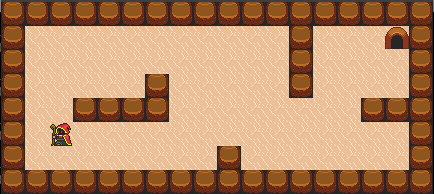
\includegraphics[width=0.5\textwidth]{./figures/experiment1}
\caption{GAME }
\label{experiment1}
\end{figure}

Experiment 1 update H

First H

TODO Insert Hypothesis here

Last H after XX iterations. 

TODO Insert Hypothesis here

% \subsection{Evaluation Methods}

Converge to optimal policy faster than Q-learning.

\begin{figure}[!htb]
\centering
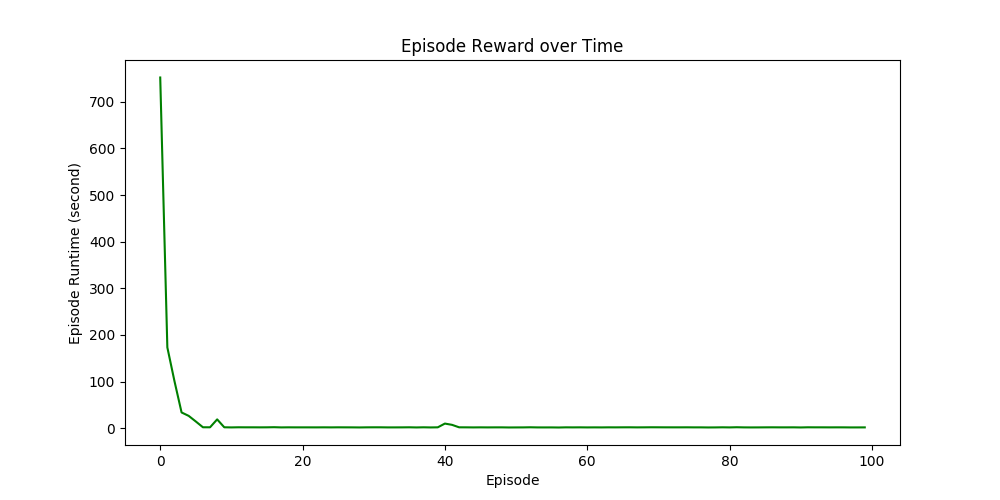
\includegraphics[width=1.0\textwidth]{./figures/placeholder}
% 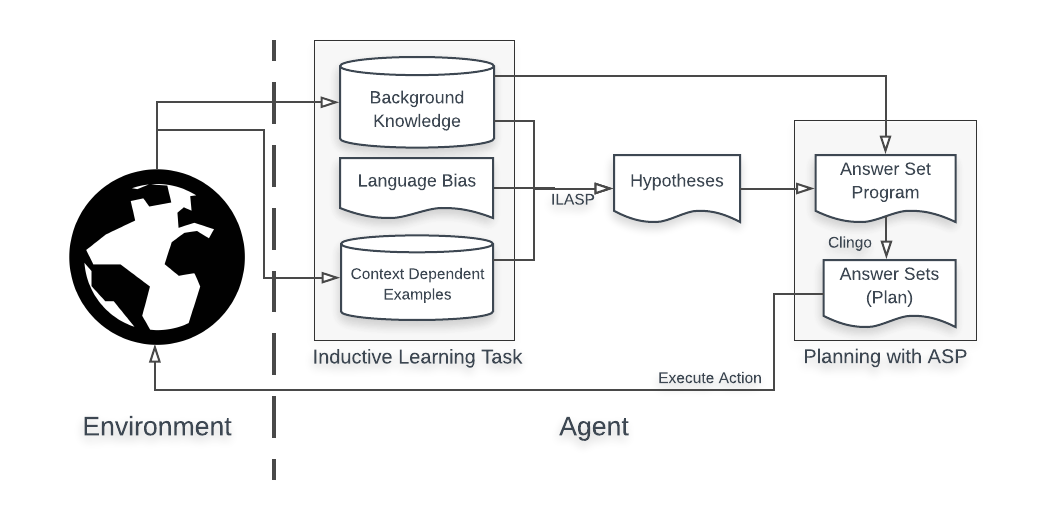
\includegraphics[width=10cm, height=9cm]{./figures/architecture}
\caption{PLACEHOLDER}
\label{proposed_architecture}
\end{figure}
    


\subsection{Experiment2}

The first experiment might not be a fair comparision between our algorithm and Q-learning, since our algorithm has extra information about the surrounding information.
In order to have the same assumptions, we use function approximation for Q-learning. 
Linear function approximation. 

\begin{figure}[!htb]
\centering
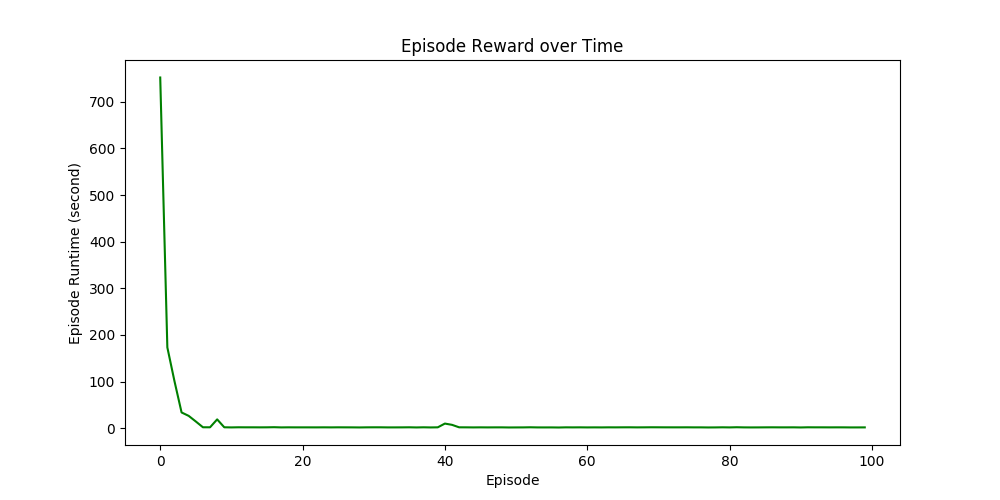
\includegraphics[width=1.0\textwidth]{./figures/placeholder}
% 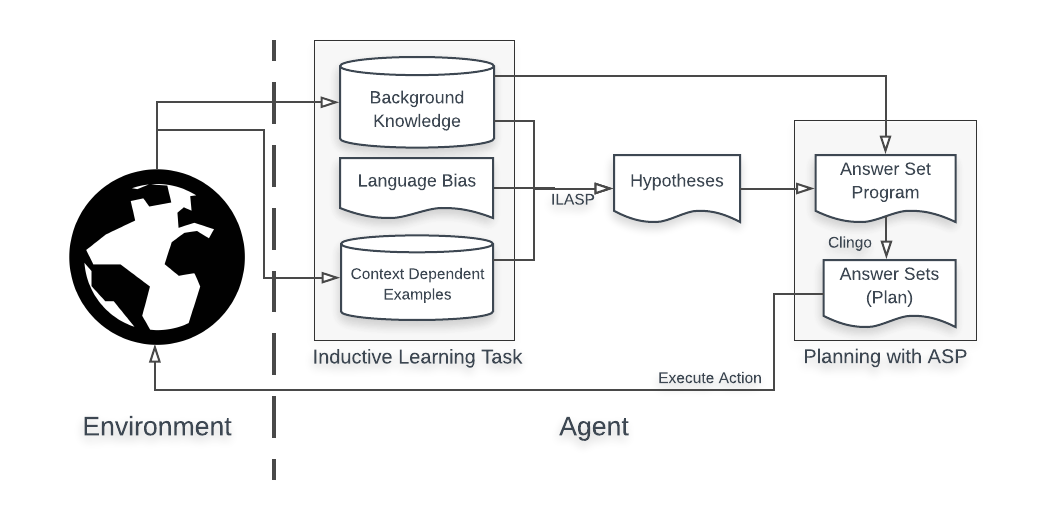
\includegraphics[width=10cm, height=9cm]{./figures/architecture}
\caption{PLACEHOLDER}
\label{proposed_architecture}
\end{figure}
    

\subsection{Experiment3}
Experiment 3 Optimal path learning
This experiment is conducted to see if the agent does not get stuck on a suboptimal path. 

The game is designed such that 

Teleport. 

\begin{figure}[!htb]
\centering
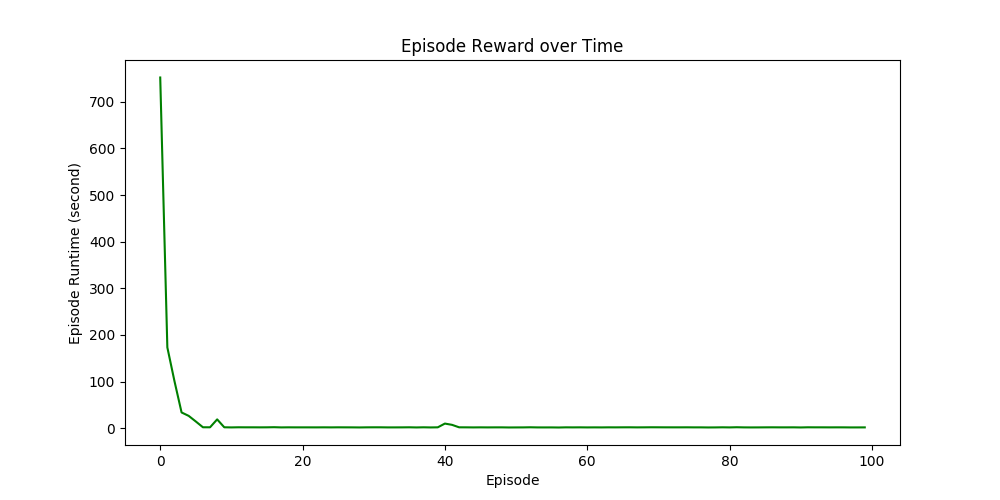
\includegraphics[width=1.0\textwidth]{./figures/placeholder}
% 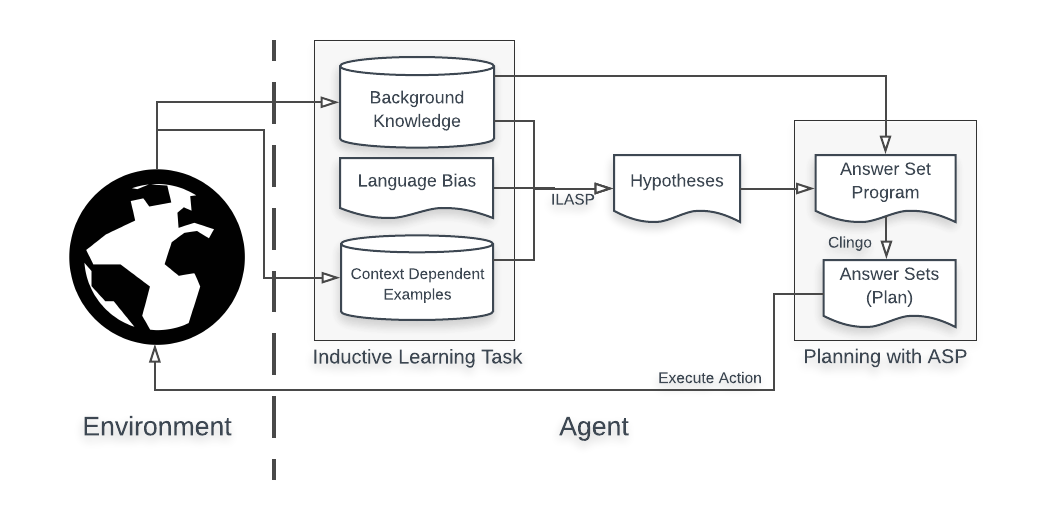
\includegraphics[width=10cm, height=9cm]{./figures/architecture}
\caption{PLACEHOLDER}
\label{proposed_architecture}
\end{figure}
    

\section{Transfer Learning Evaluation}
\label{transfer_learning}

\subsection{Experiment4}

\begin{figure}[!htb]
\centerline{
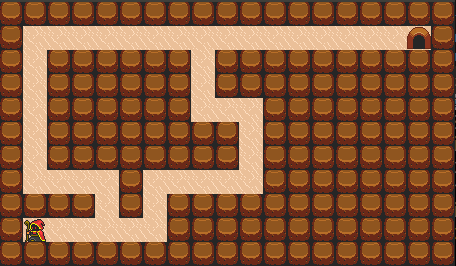
\includegraphics[width=0.5\textwidth]{./figures/experiment4_before}
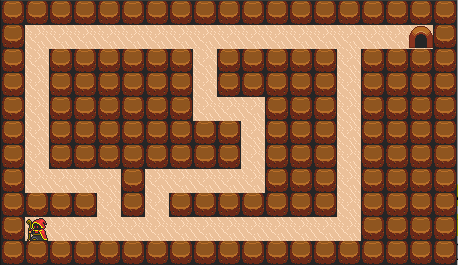
\includegraphics[width=0.5\textwidth]{./figures/experiment4_after}
}
\caption{Before (left) and after (right) transfer learning}
\label{experiment4}
\end{figure}    

Finally, we investigated the potentials of transfer learning betweeen similar environments. 

The goal position is the same as in the first game, but the routes to the goal is different. 

Experiment 4 Transfer learning 
    1 update B
    2 update H

\begin{figure}[!htb]
\centering
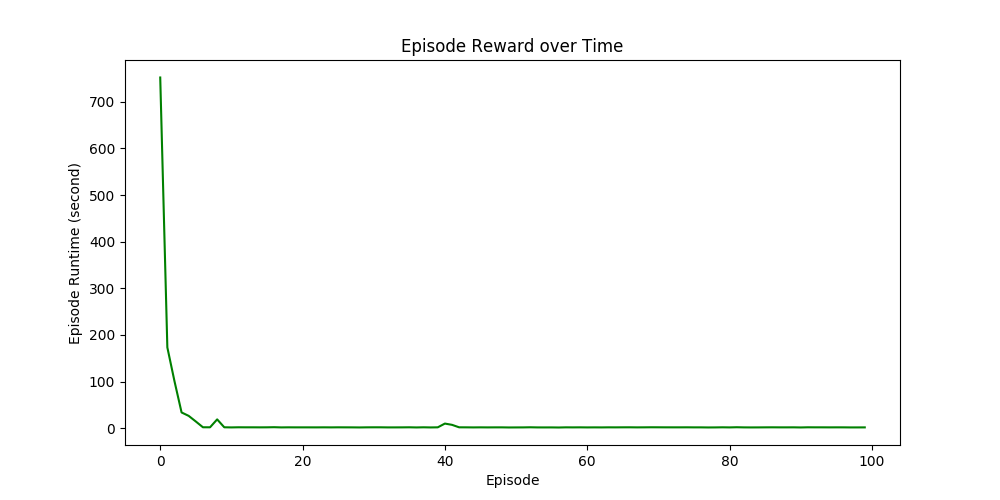
\includegraphics[width=1.0\textwidth]{./figures/placeholder}
% 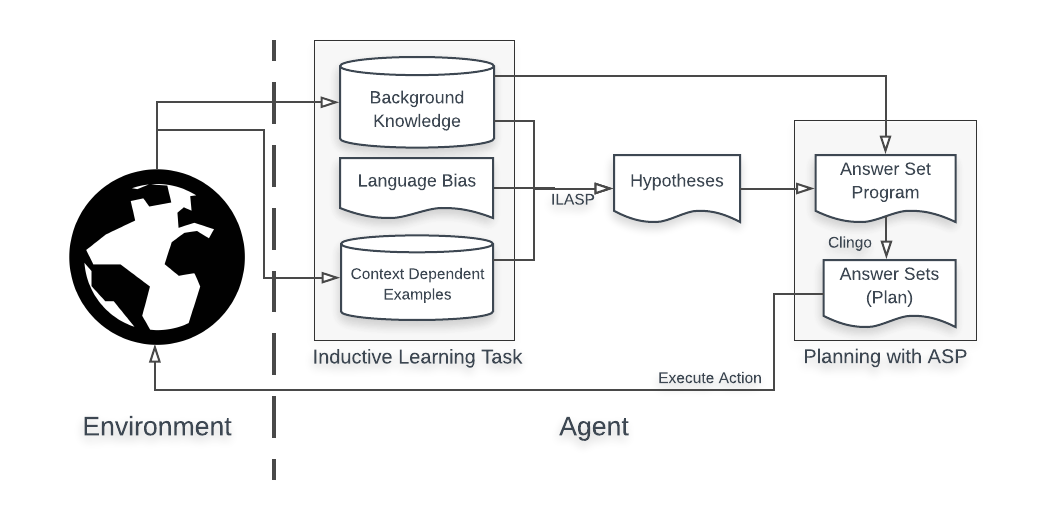
\includegraphics[width=10cm, height=9cm]{./figures/architecture}
\caption{PLACEHOLDER}
\label{proposed_architecture}
\end{figure}


\subsection{Results}

\subsection{Discussion}
\subsubsection{Strengths}

\subsection{Limitations}

You have to define the search space for H

Learning ILASP is known to be less scalable. 

ILASP learning is quite slow